% !TEX encoding = UTF-8 Unicode
\documentclass[../天体物理基础.tex]{subfiles}
\begin{document}
\section{星际介质与恒星形成}
分布在星际空间的物质,主要包括星际气体、星际尘埃、宇宙线和星际磁场。在银河系中,星际物质的质量约占银河系恒星质量的$10\%$,主要分布在距离银道面约$1000\,\mathrm{ly}$的范围内。

\subsection{星际气体和星际尘埃}
基本成分:
\begin{table}[!htbp]
\centering
\caption{星际气体和星际尘埃的基本成分}
\begin{tabular}{c c c}
\hline
性质 & 星际气体 & 星际尘埃\\
\cline{1-3}
质量百分比 & $99\%$ & $1\%$\\
\cline{1-3}
组成 & $70\%{}^{}\mathrm{H},28\%{}^{}\mathrm{He}$,其余${}^{}\mathrm{N,Ne,Na}$ & 冰、硅、石墨等固体粒子\\
\cline{1-3}
粒子数密度 & $10^{-4}\text{\textendash}10^{6}\,\mathrm{cm^{-3}}$ & $10^{-13}\,\mathrm{cm^{-3}}$\\
\cline{1-3}
质量密度 & $10^{-24}\,\mathrm{g\cdot cm^{-3}}$ & $10^{-27}\,\mathrm{g\cdot cm^{-3}}$\\
\cline{1-3}
温度 & $20\,\mathrm{K},100\,\mathrm{K},10000\,\mathrm{K},\mathrm{H}_{2},\mathrm{H\,\uppercase\expandafter{\romannumeral1}},\mathrm{H\,\uppercase\expandafter{\romannumeral2}}$ & $10\text{\textendash}20\,\mathrm{K}$\\
\cline{1-3}
研究手段 & 星际吸收线、氢 21 厘米谱线,分子谱线 & 星际消光和红化、星际极化、红外热辐射\\
\hline
\end{tabular}
\label{}
\end{table}

\subsubsection{星际气体}
星际气体的组成元素主要是氢元素。星际气体的空间分布不均匀,不同环境下 H 的存在方式不一样。
\begin{table}[!htbp]
\centering
\caption{不同成分的星际介质}
\begin{tabular}{c c c c c}
\hline
成分 & 观测证据 & 温度 $\left(\,\mathrm{K}\right)$ & 数密度$\left(\mathrm{cm^{-3}}\right)$ & 质量百分比\\
\cline{1-5}
分子云 & 红外辐射、紫外吸收线、$\mathrm{CO}$射电和红外辐射 & $10\text{\textendash}50$ & $10^{2}\text{\textendash}10^{9}$ & $40\%$\\
\cline{1-5}
$\mathrm{H\,\uppercase\expandafter{\romannumeral1}}$区 & 21 厘米谱线,紫外吸收线 & $50\text{\textendash}100$ & $1\text{\textendash}50$ & $40\%$\\
\cline{1-5}
$\mathrm{H\,\uppercase\expandafter{\romannumeral2}}$区 & 光学和红外发射线、射电连续辐射 & $10^{4}$ & $10\text{\textendash}10^{4}$ & 极少\\
\cline{1-5}
云际气体 & 21 厘米谱线 & $7000\text{\textendash}10^{4}$ & $0.2\text{\textendash}0.3$ & $20\%$\\
\cline{1-5}
云际冕气 & X 射线辐射 & $10^{6}$ & $10^{4}\text{\textendash}10^{-3}$ & $0.1\%$\\
\hline
\end{tabular}
\label{}
\end{table}

\begin{figure}[!htbp]
\centering
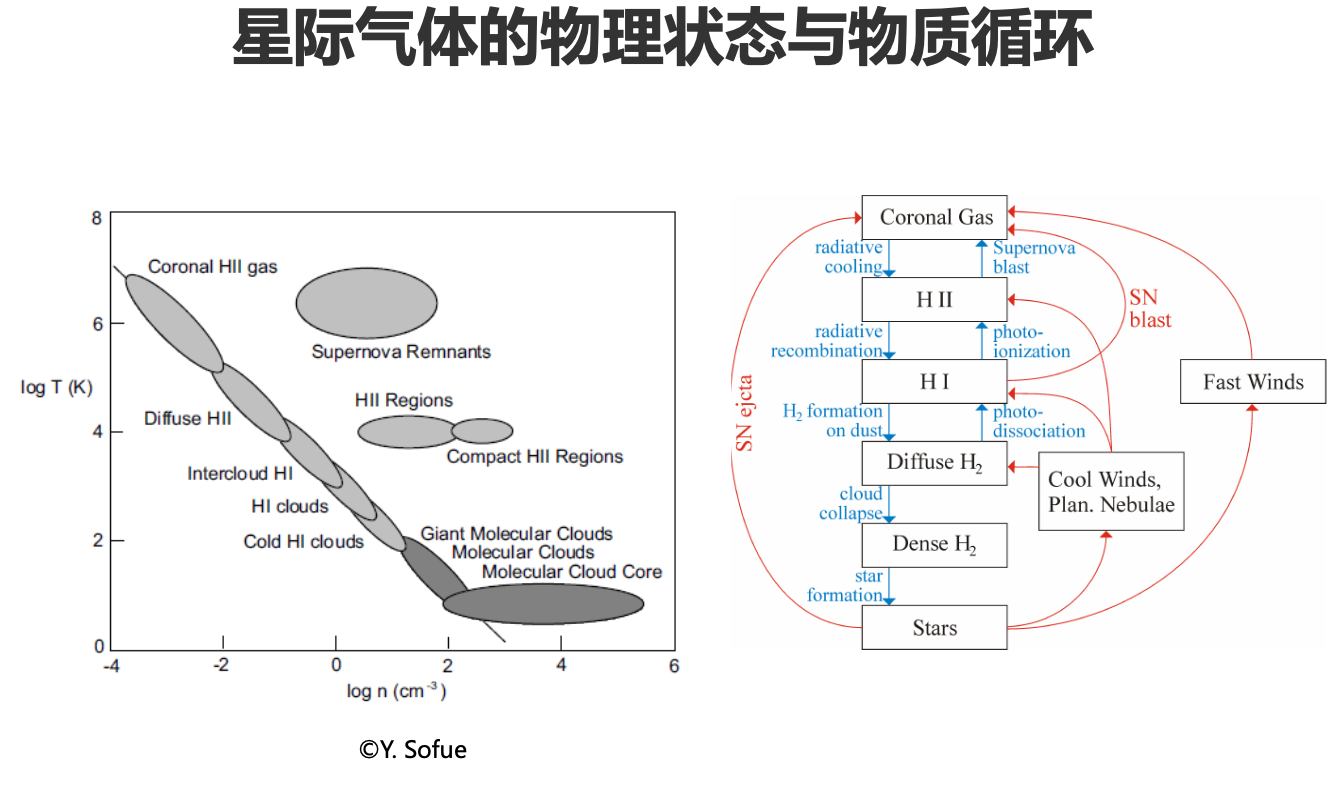
\includegraphics[width=11cm]{figures/figure3_1.png}
\captionsetup{justification=raggedright, singlelinecheck=false}
\caption{星际气体的物理状态和物质循环。}
\label{星际气体的物理状态和物质循环。}
\end{figure}

\subsubsection{电离氢气体}

发射星云:被高温恒星的紫外辐射电离的星际物质,也被称为 H\,\uppercase\expandafter{\romannumeral2} 区

具有容许和禁戒发射线,颜色偏红,典型温度$\sim8000\,\mathrm{K}$

比如$\mathrm{O}$型附近的斯特龙根球。

\subsubsection{中性氢气体}

星际吸收线:星际气体中的原子受恒星紫外光子的电离而产生吸收线。由于星光可能穿过多块气体云,可能会出现多重吸收线。

星际气体低温$\to$窄吸收线

\subsubsection{分子氢气体}

暗星云中心区域的射电观测无法探测到 21 厘米谱线。后来人们认识到暗星云主要由分子氢构成,加上少量尘埃和复杂分子。

示踪分子:氢分子不发射射电辐射,但是其他分子发射线大部分由氢分子的热运动碰撞激发产生。如利用$\rm CO$分子的$\rm 2.6mm$射电辐射可以研究氢分子的分布

分子云:通过对$\rm CO$分子的观测,发现星际分子聚集成团而形成分子云,质量$10^{6}\,M_{\odot}$,直径$600\,\mathrm{ly}$,密度$10^{3}\text{\textendash}10^{5}\,\mathrm{cm^{-3}}$

分子云占据银盘内大约$1\%$的空间,质量大约占星际气体总质量的$50\%$

巨分子云:质量$10^{6}\,M_{\odot}$,直径$300\,\mathrm{ly}$,温度$20\,\mathrm{K}$,数密度$100-300\rm cm^{-3}$,寿命$10^7-10^8\rm yr$。大约$10\%$的分子云足够致密,可以形成恒星

\subsubsection{星际尘埃}

星际尘埃对星光的散射截面随波长的变化而不同
\begin{align}
\sigma_{\lambda}\propto{}\frac{a^{3}}{\lambda},&\lambda\ge a,\\
\sigma_{\lambda}\propto{}a^{2},&\lambda\ll a.
\end{align}
因此尘埃对蓝光吸收和散射较多而对红光散射较少,导致星际消光和红化。

成分为硅或石墨颗粒,外面被冰或二氧化碳包裹

星光偏振现象$\to$尘埃呈长条形(?)

部分形成于红巨星的外层大气,在恒星演化晚期被吹向星际空间

星际尘埃提供了原子聚集形成分子的场所,并屏蔽了星光中的紫外线使分子免遭瓦解。

还有催化剂的作用

星际尘埃的观测:

光学观测:反射星云和暗星云

反射星云:星云通过尘埃反射附近的热星的光而发光,颜色偏蓝

暗星云:大量尘埃阻挡了星云内部或恒星后面的星光

红外观测:尘埃的热辐射。尘埃粒子受宇宙线和附近热星辐射的加热,温度可以达到$100\,\mathrm{K}$,产生红外热辐射。

\subsection{恒星形成}

\subsubsection{简单分析}

银河系内恒星总质量$5\times10^{10}\,M_{\odot}$,年龄$10^{10}\,\mathrm{yr}$,因此银河系平均恒星诞生率$5\,M_{\odot}\mathrm{yr^{-1}}$.

O 型星寿命约$10^{6}\,\mathrm{yr}$,是最近形成的天体,观测 O 型星确定目前的恒星诞生率为$1.65\,M_{\odot}\mathrm{yr^{-1}}$.

康德{}-{}拉普拉斯星云说:
太阳系起源于旋转的星云,由于冷却凝缩,星云旋转速度加快,呈扁平状,当离心力超过引力时逐渐分裂出许多环状物。星云中心部分凝聚成太阳,各个环状物碎裂并凝结成围绕太阳运行的行星。

后来人们逐渐认识到,恒星形成与分子云的引力坍缩有关。

星云质量足够高时,引力超过热运动提供的压力,就会引起星云坍缩。极限质量被称为金斯质量。动能$\text{K}=\dfrac{3}{2}Nk_{\text{B}}T$,势能$\text{U}\sim-\dfrac{3}{5}\dfrac{\text{G}M^{2}}{R},2\text{K}<\left\vert{}\text{U}\right\vert{}$时星云坍缩。

金斯判据只适用于均匀分布的气体。实际上气体的状态和环境十分复杂,需要考虑的因素包括星系产生的潮汐力,分子云的转动、湍动和磁场,分子云的形态等等。

位力定律分析:

无粘性流体的运动方程为:
\begin{align}
\rho\frac{\mathrm{d}\boldsymbol{u}}{\mathrm{d}t}&=-\nabla{}P-\rho\nabla\phi_{g}+\frac{1}{c}\boldsymbol{J}\times\boldsymbol{B}.\\
\rho\frac{\mathrm{d}\boldsymbol{u}}{\mathrm{d}t}&=-\nabla P-\rho\nabla\phi_{g}+\frac{1}{4\pi}\left(\boldsymbol{B}\cdot\nabla \boldsymbol{B}\right)-\frac{1}{8\pi}\nabla{}\left\vert{}\boldsymbol{B}\right\vert{}^{2}.
\end{align}
不考虑外界压强,即自引力主导下,方程转化为
\begin{equation}
\frac{1}{2}\frac{\partial{}^{2}I}{\partial{}t^{2}}=2T+2U+W+M,
\end{equation}
其中转动惯量$I=\int\rho\left\vert{}\boldsymbol{r}\right\vert{}^{2}\mathrm{d}^{3}x$,动能$T=\dfrac{1}{2}\int\rho\left\vert{}\boldsymbol{u}\right\vert{}^2\mathrm{d}^{3}x$,热能$U=\dfrac{3}{2}\int nkT\mathrm{d}^3x$,引力势能$W=\dfrac{1}{2}\int\rho\phi_{g}\mathrm{d}^{3}x$,磁能$M=\dfrac{1}{8\pi}\int\left\vert{}\boldsymbol{B}\right\vert{}^{2}\mathrm{d}^{3}x$.

气体云在引力坍缩时,$\dfrac{1}{2}\dfrac{\partial{}^{2}I}{\partial{}t^{2}}\approx-\dfrac{\text{G}M^{2}}{R}$.坍缩时标
\begin{equation}
t_{\text{ff}}\sim\left(\frac{1}{4\pi{}G\rho}\right)^{\frac{1}{2}}\sim5\times10^{5}\left(\frac{n}{10^{4}\,\mathrm{cm^{-3}}}\right)^{-\frac{1}{2}}\,\mathrm{yr}.
\end{equation}

星云坍缩触发机制:

1. 激波压缩:超新星爆发、热星辐射、银河系旋臂转动等过程产生激波,激波压缩周围星云,使其密度增大,触发恒星形成,其过程类似链式反应。

2. 星云与旋臂区域碰撞,由于旋臂密度更高,星云坍缩,产生恒星。

恒星形成的 Kennicutt-Schmidt 定律
\begin{figure}[!htbp]
\centering
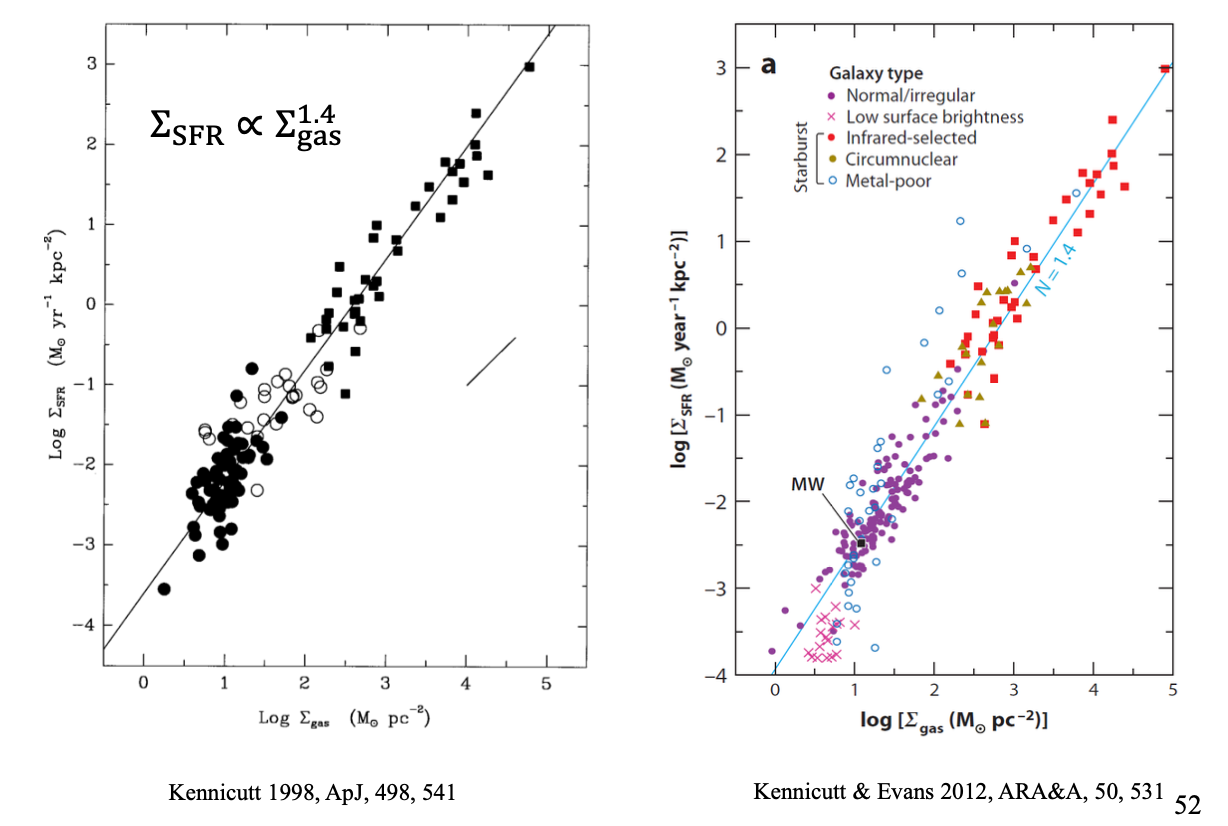
\includegraphics[width=13cm]{figures/figure3_2.png}
\captionsetup{justification=raggedright, singlelinecheck=false}
\caption{恒星形成的 Kennicutt-Schmidt 定律}
\label{}
\end{figure}

初始质量函数 (Initial Mass Function): 单位体积内形成的恒星的相对数目在质量上的分布,可以表示成
\begin{equation}
\xi\left(m\right)\mathrm{d}m=\xi_{0}m^{-\alpha}\mathrm{d}m,
\end{equation}
其中$m=\dfrac{M}{M_{\odot}}$. E.Salpeter 最早提出初始质量函数的概念,并发现$\alpha=2.35$.

\subsubsection{恒星形成理论}

质量越大的恒星,演化到主序的时间越短,主序上的位置越高

\paragraph{低质量恒星的形成}~{}

1. 分子云和云核

最初大体处于流体静力学平衡,分子云缓慢旋转和收缩,引力能转化为动能进而转化为内能,产生辐射。由于云核光学薄,热量可以不受阻碍地逃逸,云核等温坍缩。

由于旋转速度加快,此时分子云可以分裂成更小的云核,云核进一步收缩和分裂,导致密度上升,金斯质量下降。核心逐渐变得不透明,趋向绝热坍缩,温度迅速上升,金斯质量增大,云核停止分裂,开始坍缩。

2. 云核引力坍缩

坍缩时标
\begin{equation}
\frac{\mathrm{d}^{2}r}{\mathrm{d}t^{2}}=-\frac{\mathrm{G}M_{r}}{r^{2}}\to t_{\text{ff}}=\left(\frac{3\pi{}}{32\mathrm{G}\rho}\right)^{\frac{1}{2}}.
\end{equation}

密度均匀的星云同步坍缩,中心致密星云自内向外坍缩

由于角动量大小的差异,中心区域的气体直接落入引力势阱中形成原恒星,而外层气体形成一个围绕中心区域旋转的扁平吸积盘。

3. 原恒星的吸积与成长

原恒星通过吸积盘快速吸积气体。转动和磁场产生的喷流成功带走吸积盘气体角动量,进而吸积盘可以吸附质量。内部完全对流,赫罗图上沿林中四郎线演化

4. 主序前星的形成与演化

吸积率下降,外向流张角变大,原恒星质量不再实质增长,成为主序前星,但内部温度还未升高到$\rm H$的点火温度。原恒星以热时标收缩。中心星的辐射和星风驱散部分吸积物质,其余部分形成原行星盘。

5. 零龄主序

核心的热核反应开始进行,光度约为目前太阳光度的三分之二

\paragraph{大质量恒星形成的问题}~{}

观测方面,新生的大质量恒星深埋在致密的云核中,观测时标短。此外,紫外辐射对环境的破坏导致很难追溯初始形成条件。理论方面,恒星的辐射加热、电离周围气体会阻碍其坍缩和吸积。

模型有三种,

1. 云核直接坍缩

小质量恒星形成模型的放大版本,$M_{\text{J}}>10\,M_{\odot}$,辐射加热或湍动、磁场主导内部压力。但是湍动作用未知,尚未观测到大质量恒星前核。

2. 竞争吸积

$M_{\text{J}}\sim0.5\,M_{\odot}$,处于引力优势位置的原恒星更容易通过吸积周围的气体生长,但这样提供的恒星形成效率低。

3. 小质量原恒星的并合,要求原恒星中心数密度达到$10^{8}\,\mathrm{pc^{-3}}$.

\paragraph{极小质量恒星可能的形成机制}~{}

湍动分子云核的分裂

多个原恒星胚胎相互作用时被抛出的较小的个体

原恒星盘的碎裂

原恒星核的光致腐蚀

\subsubsection{其他问题}

形成恒星的云核的角动量比恒星大几个量级,说明角动量转移到多星系统的轨道角动量或通过吸积盘向外转移

星云的转动坍缩往往伴随多星系统的形成

转动星云在坍缩过程中会形成围绕原恒星旋转的环或盘。




O、B 型恒星表面温度高能产生大量紫外 ($\lambda<912\,\si{\angstrom}$) 光子电离氢,产生$\mathrm{H\,\uppercase\expandafter{\romannumeral 2}}$区。如斯特龙根球就是年轻 O、B 型恒星周围存在的电离氢区。光致电离产生的大量自由电子之间相互频繁碰撞,建立电子气的平衡态速度分布。



% \printbibliography

\end{document}